\textbf{Problema 4.} (2.5 puntos) (2.5 puntos) Considérese un circuito eléctrico en serie, formado por una resistencia
$R$, un condensador de capacidad $C$, una bobina de autoinducción $L$ y una batería de tensión
constante $V_0$ . En el instante de tiempo $t = 0$ se cierra el interruptor, con lo que comienza a
circular corriente en el circuito (ver figura). Entonces, la intensidad de corriente, $i$, es función del
tiempo $t$ transcurrido tras el cierre del interruptor, y además, la función $i(t)$ satisface el problema

\begin{equation*}
    L\frac{di}{dt} + R i + \frac{1}{C} \int_0^t i(\tau) d\tau = V_0 \hspace{10pt} (t > 0), \hspace{20pt} i(0) = 0.
\end{equation*}

Usando el método de la transformada de Laplace, encontrar la función $i(t)$ en cada uno de los
tres casos siguientes:

\begin{enumerate}[i)]
    \item $w_1^2 = \frac{1}{LC} - \frac{R^2}{4L^2} > 0$.
    \item $w_2^2 = \frac{R^2}{4L^2} - \frac{1}{LC} > 0$.
    \item $\frac{R^2}{4L^2} = \frac{1}{LC}$.

\end{enumerate}\\




\begin{center}
    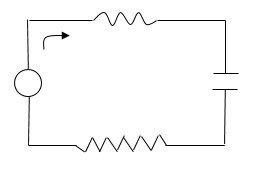
\includegraphics[width=5cm]{files/img}
\end{center}



\underline{Observación}: Introduzca también (en los tres casos) la constante $p = R/ (2L)$. Además, puede
hacer uso, si es necesario, de la tabla de transformadas de Laplace que se adjunta con la prueba.